\subsection{Raspberry Pi (TM)}
\label{sec:rpi}

% Tasks and did we reach them?
% 2 Components -> main and servo
% terminal problems: different than linux (device files)
% problems and solution?

\subsubsection{General information}
The Raspberry Pi is one of the ECUs used in the setup. There are three Raspberry Pis placed on the model car in total, whereas two of them are Raspberry Pis of the first generation and one is a Raspberry Pi of the second generation. For our purpose we only need one of them. \\

The main goal of the Raspberry Pi is to receive commands from the second ECU which is the PandaBoard and control the servos with the given command. Therefore, it is connected via a usb-to-uart bridge with the \textit{pololu maestro} servo controller board which in turn is connected to the braking and the steering servos. This can be seen in figure \ref{fig:arch}. \\

Since the Raspberry Pi has IO pins itself, it would have been possible to directly connect the servos to the Raspberry Pi and completely give up the \textit{pololu} board. However, there are mainly two reasons for not doing so. Firstly, because in this lab course we want to simulate a real car which usually consists of many different ECUs that have to work together. Secondly, because the \textit{pololu} board has more power for controlling the servos than the Raspberry Pi. 


\subsubsection{Task description and solutions}
From the initial task description we can derive the following tasks related to the Raspberry Pi component:

\begin{itemize}
    \item \textbf{T1}: Install Genode with Fiasco.OC
    \item \textbf{T2}: Implement ProtoBuf by Google
    \item \textbf{T3}: Develop MQTT client
    \item \textbf{T4}: Connect with servo controller board
    \item \textbf{T5}: Implement Genode Servo controller application
    \item \textbf{T6}: Convert control commands into concrete servo values
    \item \textbf{T7}: Read sensor values (optional)
\end{itemize}

\paragraph{\textbf{T1}} Since the complete project is based on Genode with Fiasco.OC, the first task was obviously to install the operating system on the Raspberry Pi. There have been many issues with this task which is described in detail in section \ref{sec:pi-problems}. Shortly summarized we were not able to build the operating system for the Raspberry Pi until the last two weeks of the lab course. For this reason we came up with a complete Linux-based solution at interim. The Linux-based solution is explained in section \ref{sec:pi-linux}.

\paragraph{\textbf{T2}} The next two tasks are related to the message exchange between the PandaBoard and the Raspberry Pi. Originally, it was planned to use protocol buffers (ProtoBuf) by Google for the communication. ProtoBuf is a language -and platform-neutral way of serializing data comparable to XML or JSON format. However, the main advantage is its binary format which allows really fast parsing and shrinks messages to a minimum size. We have already started by specifying a \textit{.proto} file for the message type. However, afterwards we came to the conclusion that ProtoBuf is not really necessary and can be replaced by mqtt with messages in plain-format. This has mainly two reasons. Firstly, because the messages sent from the PandaBoard do only consist of a few characters and also have a really simple format. Therefore, it is absolutely fine to use plain-format. Secondly, because mqtt is already used for the communication between the simulation and the PandaBoard. Therefore, we have already a mqtt broker in our project and apart from that, we have to implement only one of the two techniques.

\paragraph{\textbf{T3}} The mqtt client is only implemented once in the project and is used by the Raspberry Pi, as well as the PandaBoard. The mqtt client is based on the mosquitto library which is already ported for Genode. The Raspberry Pi is subscribed to the topic \texttt{car-servo} at which the PandaBoard publishes its messages. A description of the message format can be found in section \ref{sec:mqtt-car-servo}. After receiving the messages, the Raspberry Pi only checks for valid input values and controls the servos accordingly.

\paragraph{\textbf{T4}} The next task was to connect the Raspberry Pi with the \textit{pololu maestro} servo controller board. Obviously, this is necessary in order to be able to control the connected servos. The \textit{pololu} boards are quite comfortable in the way that they support a serial connection. Therefore, we only had to plug the usb-to-uart bridge into the Raspberry Pi.

\paragraph{\textbf{T5}} The Genode servo controller application is the main task regarding the Raspberry Pi. Is is completely described in section \ref{sec:pi-genode}.

\paragraph{\textbf{T6}} Another obvious task was to convert the abstract control commands coming from the simulation into concrete servo values that can be used in order to control the servos. However, in our opinion it is more meaningful to separate this task from the rest of the tasks of the Raspberry Pi. That is because the Raspberry Pi is actually only responsible for controlling the servos, but not for the core logic. Therefore, we shifted this task to the PandaBoard and expect mqtt messages that are already in the right servo format. 

\paragraph{\textbf{T7}} The last task regarding the Raspberry Pi was to read sensor values of the model car which could be steering angles or wheel speeds, for instance. This task was marked as optional in the initial task description. Actually, this task is required in order to close the loop of the HIL-testbed. However, due to fact that the model car does currently not contain any sensors, we were not able to achieve this task.


\subsubsection{Linux-based solution}
\label{sec:pi-linux}
One major problem, we experienced during the development, was that we were not able to build the Genode operating system for the Raspberry Pi and it was not predictable whether this would be possible until the end of the lab course, at all. For this reason we decided to implement all tasks of the Raspberry Pi on a Linux basis as a backup solution. \\

The used Linux distribution was a \textit{Raspbian} image copied onto a sd-card that was plugged into the Raspberry Pi. Of course, Linux comes with a high overhead for what is actually required in order to control some servos. Indeed, this is one of the main reasons why we use a microkernel-based solution, at all. However, Linux does also simplify a lot of things during the development. \\

One of those simplifications is for example an ssh server. After changing something in the program code, we could simply transfer the updated code to the Raspberry Pi via ssh or even program directly on the Raspberry Pi. With Genode, this does always require to build a new image, copy the image onto the sd-card and reboot the Raspberry Pi. \\

A second simplification is the way how Linux handles its serial connections. After connecting the \textit{pololu} board with the Raspberry Pi, the board appears inside the \texttt{/dev} directory and we can simply use normal file operations like \texttt{open, read} and \texttt{write} in order to control the servos that are connected to the \textit{pololu} board. \\

A last advantage of Linux over Genode is the ability to easily run a mosquitto server beside of the main program. The mosquitto server is required for mqtt. The good thing about running the mosquitto server directly on the Raspberry Pi is that we do not have to struggle with correctly setting up the network since the Raspberry Pi is already in the same network as the PandaBoard. \\

The source code itself is similar to the Genode version with only a few differences. One is for example that there is only one task for the whole program under Linux. In Genode it is common to separate different components into different tasks which requires a few changes in the source code, as well. For the header and source files of the mqtt client it was possible to reuse them in the exact same way in the Genode version. As already mentioned, the only big difference compared to the Genode version is the way how commands via the serial connection are sent. In Genode this requires the usage of a so-called \texttt{terminal} connection which is described in detail in section \ref{sec:pi-genode}.

\subsubsection{Genode application}
\label{sec:pi-genode}
The Genode application is the main task regarding the Raspberry Pi. One of the main reasons for using a microkernel-based operating system like Genode is the minimal overhead of the system itself. The disk image file does basically only contain programs and libraries that are really required in order to fulfill the task and nothing more. Especially in embedded systems, where computing power and memory are limited, this is a big advantage over "normal" operating systems like Linux. \\

The relevant components of the Genode application running on the Raspberry Pi are illustrated in figure \ref{fig:pi-genode}. As one can see, the application consists of two different components that are connected via IPC. This is the usual procedure in microkernel-based operating systems like Genode. The advantage of seperating tasks into different components is that a failing component usually only leads to a crash of that individual component, but not of the whole program. \\

\begin{figure}[h]
    \centering
    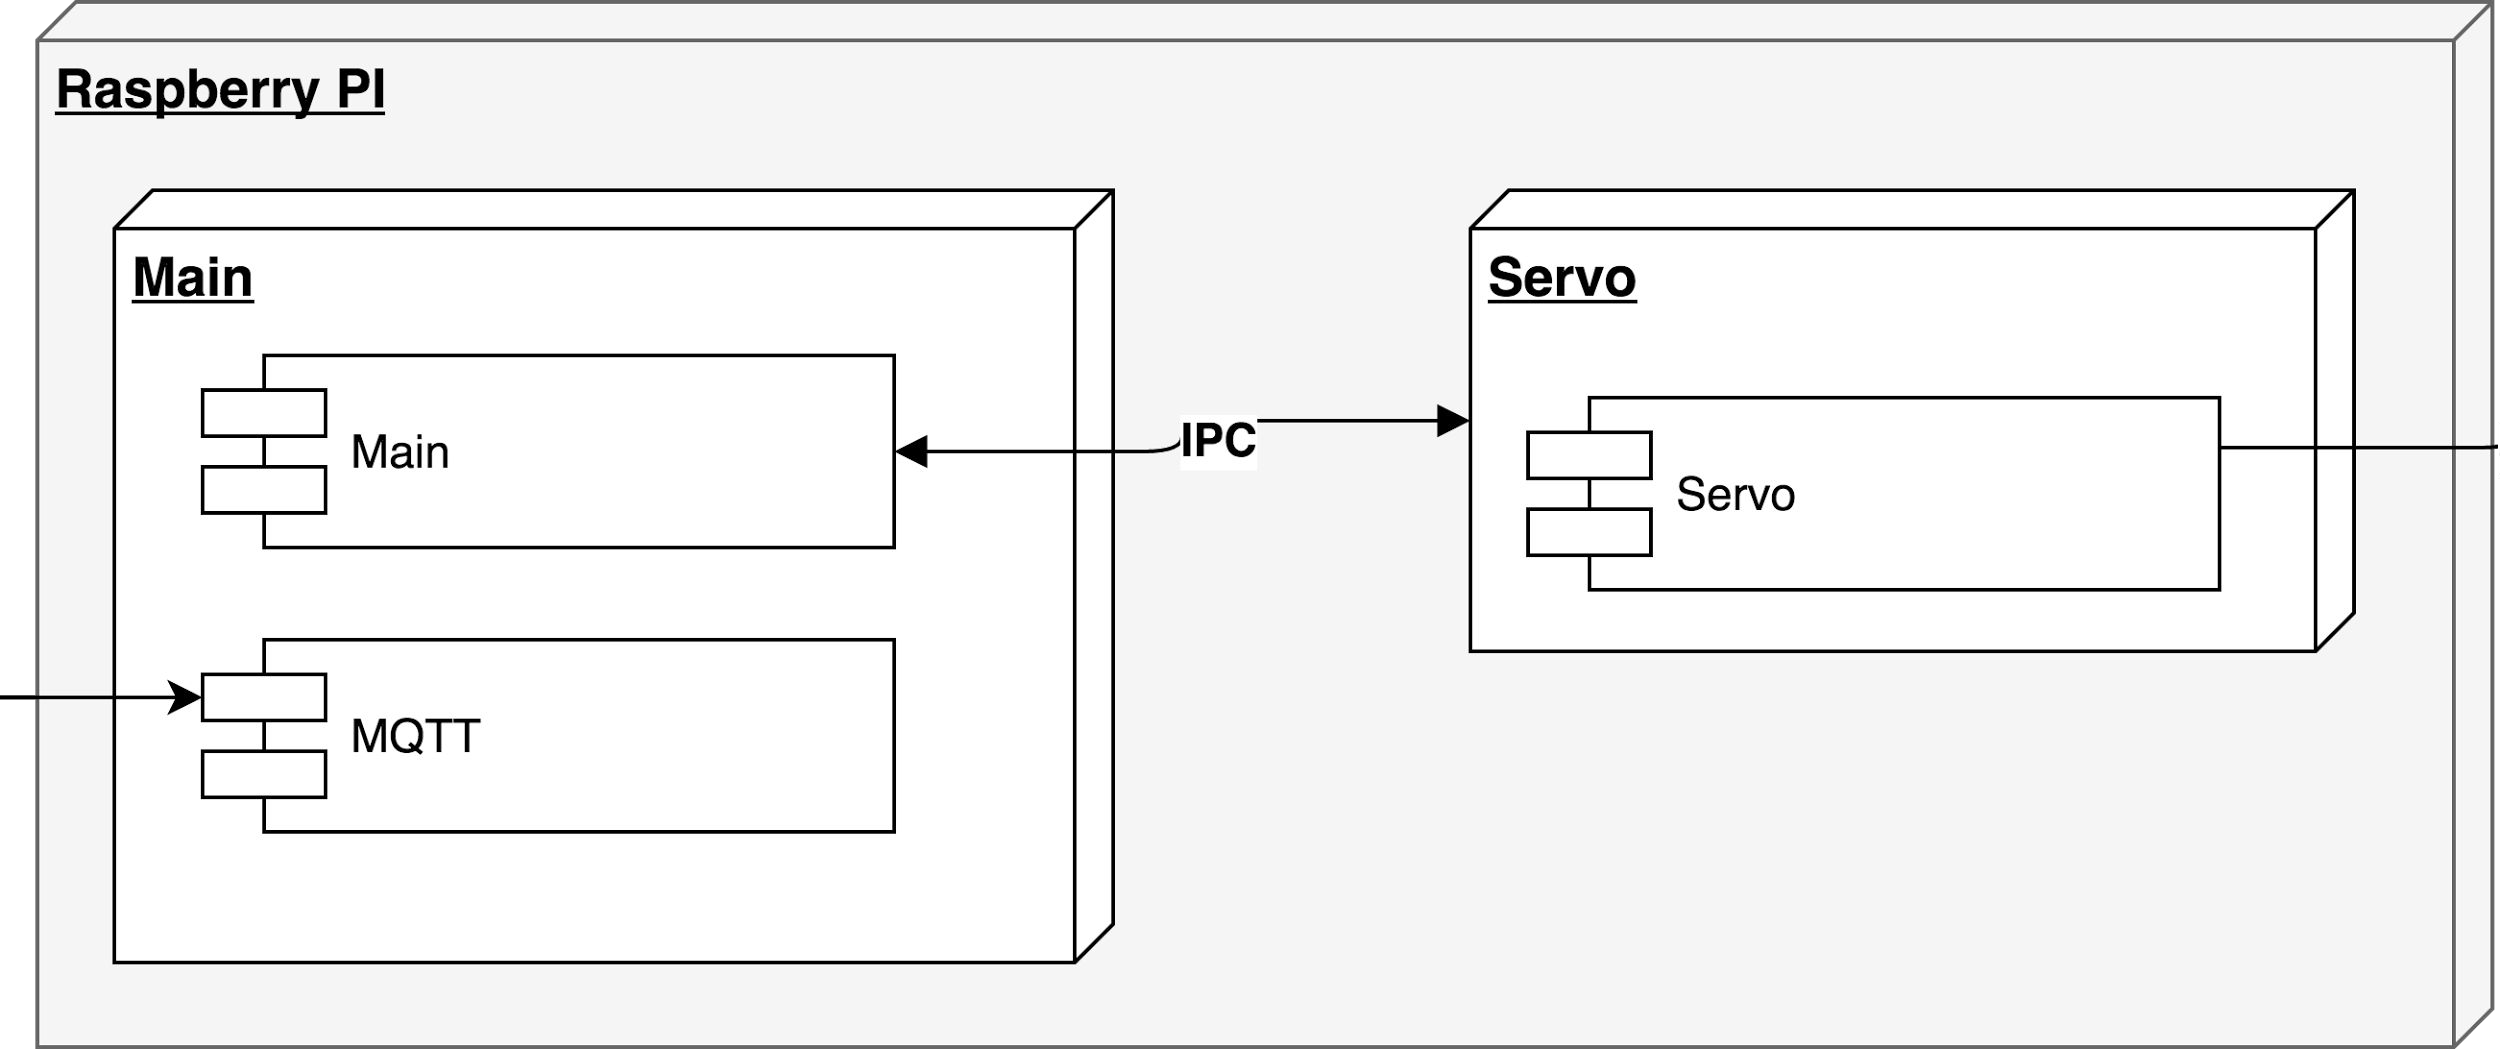
\includegraphics[width=0.7\linewidth]{images/pi}
    \caption{Genode components of the Raspberry Pi}
    \label{fig:pi-genode}
\end{figure}

The \texttt{Main} component fulfills the following functions:

\begin{itemize}
    \item Setup the network
    \item Subscribe to \texttt{car-servo} mqtt topic
    \item Receive mqtt messages
    \item Call servo component
\end{itemize}

The relevant source code file is \textit{main.cc} placed in \texttt{src/rpi\_component/rpi/} according to the source code structure shown in figure \ref{fig:structure}. \\

The \texttt{Servo} component on the other hand is responsible for sending the received commands to the \textit{pololu} board via the serial connection. The relevant files for the \texttt{Servo} component are the header files \textit{client.h, connection.h} and \textit{servo\_session.h} placed in \texttt{include/servo\_session/} and the \textit{main.cc} file in \texttt{src/rpi\_component/servo/}. \\

The \textit{servo\_session.h} defines all the function names and exports them to Genode. This is already described in the API description in section \ref{sec:comp-servo}. The \textit{main.cc} file on the other hand implements all of the functions inside a \texttt{Servo\_component} struct that inherits from \texttt{Genode::Rpc\_object}. Apart from that, it implements a \texttt{Servo\_root} class that in turn inherits from \texttt{Genode::Root\_component} and is responsible for creating the session of a \texttt{Servo\_component} object. This is the usual procedure of implementing Genode objects. \\

An object of a \texttt{Terminal::Connection} is required in order to write to the serial connection. This differs from the Linux-based solution where normal file operations were possible. However, the Genode version is not really more complicated because the terminal does also provide a \texttt{write} function which behaves the same as the Linux function. Listing \ref{lst:set-target} exemplarily shows the \texttt{setTarget} function where the \texttt{write} operation can be seen. The \texttt{command} in the listing follows the \textit{pololu} compact protocol which is documented at the \textit{pololu} homepage\footnote{\url{https://www.pololu.com/docs/0J40}}. \\

\begin{minipage}{\linewidth}
\begin{lstlisting}[style=mylistings, language=c, label=lst:set-target, caption=setTarget function of the servo component]
int setTarget(unsigned char channel, unsigned short target)
{
    // check for valid input
    [...]

    // create command
    unsigned char command[] = 
        {0x84, channel, (unsigned char)(target & 0x7F), 
        (unsigned char)(target >> 7 & 0x7F)}; 

    // write command to serial connection
    if (_terminal->
        write(command, sizeof(command)) < sizeof(command)) {
            PERR("error writing");
            return -1; 
    }
    
    return 0;
}
\end{lstlisting}
\end{minipage} \\

The last important file for the Raspberry Pi is its run file (\textit{run/car\_rpi.run}) in which all build components and boot modules are defined. Apart from that, the configuration of the loaded modules is placed inside the run file and the IP address of the mosquitto servo is declared here.

